
\section{\MakeUppercase{Future Enhancement:}}
\begin{itemize}
    \item We can Integrate JavaScript to create interactive elements and dynamic behaviors within
    the generated user interfaces.
    \item The system can be extended to support multiple frontend frameworks including React,
    Angular, and Vue.js to accommodate different development environments.
    \item We can implement responsive design capabilities where generated interface
    automatically adapts to different screen sizes and devices.
    \item We can increase the elements pool to include more complex UI components such as
    calendar, navigation menus etc.
\end{itemize}
    \pagebreak

\section{\MakeUppercase{Conclusion}}
Our project has successfully developed an artificial Intelligence model that transforms hand-drawn
sketches into functional HTML/CSS code. By using transformer models, particularly the Compact
Convolutional Transformer Encoder which achieved an impressive BLEU score of 0.901. We've created a
bridge between design ideas and working prototypes. Convolution layer used in our Encoder helped to
extract the important features which reduce the size of the input and making it easier to train a model.
We built a custom Domain Specific Language to represent UI elements and their hierarchical structure,
and then created a user-friendly interface that lets users to easily customize text, images, and fonts. The
dataset generator which we created solved the training data challenge by automatically producing
required sketch and its associated DSL code. This tool helps designers and developers work faster by
turning layout drawn on paper into usable code in seconds which saves time for more creative tasks.
While our current version focuses only on static layouts, the foundation is in place for future
enhancements like adding JavaScript interactivity, supporting popular frameworks, and expanding the
available UI elements. Overall, our project demonstrates how AI can be used to create a functional code
from initial design.
\pagebreak
\section{\MakeUppercase{Appendices}} \label{sec:appendices}
   
    \subsection*{Appendix A: Project Schedule}
    \addcontentsline{toc}{subsection}{Appendix A: Project Schedule}
    \begin{figure}[H]
        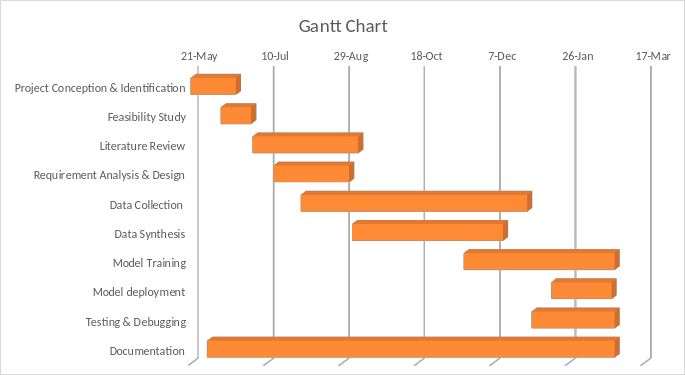
\includegraphics[width=\textwidth]{images/gantt.png}\caption{Gantt Chart}\label{fig:tabgant}
    \end{figure}

    
    \subsection*{Appendix B: \gls{dsl} Generation Rules}
    \addcontentsline{toc}{subsection}{Appendix B: DSL Generation Rules}
    \appendixnumbering{B} % For appendix Math numbering like B-1, B-2, etc.

\begin{verbatim}
1. Dictionary for Child Elements
graph={
    'root':['header','container','footer'],
    'header':['flex'],
    'nav':['navlink'],
    'logodiv':['image','text'],
    'container':['row'],
    'row':['div-3','div-6','div-9','div-12'],
    'div-3':['text','paragraph','image','card','input','button',],
    'div-6':['text','paragraph','image','card','carousel','input'
    ,'button','flex'],
    'div-9':['text','paragraph','image','card','carousel','input',
    'table','button','flex'],
    'div-12':['text','paragraph','image','card','carousel','input',
    'table','button','flex'],
    'flex':['text','button'],
    'card':['text','paragraph','image','input','button','flex'],
    'footer':['text']
}
\end{verbatim}
\begin{verbatim}
2. Rules for Child Elements
rules = {
    'root': {'inOrder': True},
    'logodiv': {'inOrder': True},
    'header':{'min':1,'max':1},
    'container': {'min': 1, 'max':3},
    'row': {'combinations':True,'0': divCombinations,
    '1':divCombinations2,'proba':0.9},
    'div-3': {'min': 2, 'max': 4},
    'div-6': {'min': 2, 'max': 4},
    'div-9': {'min': 2, 'max': 4},
    'div-12': {'min': 2, 'max':4},
    'card': {'min': 2, 'max': 3},
    'footer': {'min': 1, 'max': 1},
    'nav':{'min': 1, 'max': 5},
    'flex':{'min':2,'max':4},
}
\end{verbatim}
\begin{verbatim}
3. DSL to HTML mappings = {
    "opening-tag": "{",
    "closing-tag": "}",
    "body": "\r\n {} <style>\nmax-width: 900px;
    \nmax-height: 300px !important;\n</style>\n",
    "root": "\r\n<div class=\"root\">{}</div>\r\n",
    "header": "\r\n<header class=\"header\">{}</header>\r\n",
    "nav": "\r\n<nav class=\"nav\">{}</nav>\r\n",
    "navlink": "\r\n<a href=\"#\" class=\"navlink\">[]</a>\r\n",
    "logodiv": "\r\n<div class=\"logodiv\">{}</div>\r\n",
    "container": "\r\n<div class=\"container\">{}</div>\r\n",
    "row": "\r\n<div class=\"row\">{}</div>\r\n",
    "div-3": "\r\n<div class=\"div-3\">{}</div>\r\n",
    "div-6": "\r\n<div class=\"div-6\">{}</div>\r\n",
    "div-9": "\r\n<div class=\"div-9\">{}</div>\r\n",
    "div-12": "\r\n<div class=\"div-12\">{}</div>\r\n",
    "flex": "\r\n<div class=\"flex\">{}</div>\r\n",
    "flex-sb": "\r\n<div class=\"flex-sb\">{}</div>\r\n",
    "flex-c": "\r\n<div class=\"flex-c\">{}</div>\r\n",
    "flex-r": "\r\n<div class=\"flex-r\">{}</div>\r\n",
    "text": "\r\n<div class=\"text\">{}</div>\r\n",
    "text-c": "\r\n<div class=\"text-c\">{}</div>\r\n",
    "text-r": "\r\n<div class=\"text-r\">{}</div>\r\n",
    "paragraph": "\r\n<p class=\"paragraph\">{}</p>\r\n",
    "image": "\r\n<img src=\"placeholder.jpg\" class=
    \"image\">\r\n",
    "card": "\r\n<div class=\"card\">{}</div>\r\n",
    "input": "\r\n<input type=\"text\" class=\"input\" 
     placeholder=\"Enter text\">\r\n",
    "button": "\r\n<button class=\"button\">{}</button>\r\n",
    "button-c": "\r\n<button class=\"button-c\">{}</button>\r\n",
    "button-r": "\r\n<button class=\"button-r\">{}</button>\r\n",
    "footer": "\r\n<footer class=\"footer\">{}</footer>\r\n",
    "table": "\r\n<table class=\"table\">{}</table>\r\n",
    "carousel": "\r\n<div class=\"carousel\">{}</div>\r\n"
}
\end{verbatim}
\begin{verbatim}
4. Color Mapping for each elements = {
        'paragraph': np.array([193, 188, 192]),
        'text': np.array([255, 255, 255]),
        'button': np.array([19, 247, 47]),
        'navlink': np.array([255, 0, 0]),
        'carousel': np.array([255, 165, 0]),
        'table': np.array([165, 42, 42]),
        'input': np.array([255, 159, 252]),
        'image': np.array([0, 0, 255]),
        'header': np.array([0, 255, 255]),
        'footer': np.array([154, 128, 235]),
        'card': np.array([0, 128, 128]),
    }
    \end{verbatim}
    

\pagebreak


% References (IEEE style)
\bibliographystyle{IEEEtran}  % Use IEEE bibliography style
\bibliography{refs}
\addcontentsline{toc}{section}{References}

